%%%%%%%%%%%%%%%%%%%%%%%%%%%%%%%%%%%%%%%%%%%%%%%%%%%%%%%%%%%%%%%%%%%%%%
% Lớp 10 | Bất phương trình bậc 2 một ẩn | Giải bất phương trình bậc 2 một ẩn
% Dạng 0D7?2-7: Toán thực tế  ứng dụng bất phương trình bậc 2 một ẩn
% Số câu: 13  (sinh tự động bởi tach_cau.py; từ nay thầy sửa trực tiếp file này)
%%%%%%%%%%%%%%%%%%%%%%%%%%%%%%%%%%%%%%%%%%%%%%%%%%%%%%%%%%%%%%%%%%%%%%

%%%%%%%%%%%%%%%% ĐÚNG/SAI %%%%%%%%%%%%%%%%

% nguồn: MaHoaNH_DungSai_Lop10
\begin{ex}%[0D7V2-7]%[ma:c0002a74]
	Công ty $A$ có $100$ cán bộ công nhân viên và muốn tổ chức cho toàn công ty đi Year End Party tại khu du lịch Tam Đảo, Vĩnh Phúc. Một công ty du lịch chào giá về với công ty A như sau:\\ 
	Với $40$ khách hàng đầu tiên có giá vé là $3$ triệu  đồng/người.\\
	Nếu có nhiều hơn $40$ người đăng kí đi thì cứ thêm $1$ người giá vé sẽ giảm $15\,000$  đồng/người cho toàn bộ hành khách.\\
	Gọi $x$ là số lượng cán bộ công nhân viên của công ty $A$  đăng kí thứ $41$ trở lên. Biết chi phí thực tế công ty dành cho mỗi khách hàng là $1{,}95$ triệu đồng.
	 \choiceTF
		{\True Giá vé còn lại  sau khi thêm $x$ người là $3\,000-15x$ (nghìn đồng/người)}
		{Chi phí thực tế cho chuyến đi  này là $1\,950\cdot(40-x)$ (nghìn đồng)}
		{Lợi nhuận của công ty du lịch đạt được biểu thị bằng công thức $T=15x^{2}-450x+42\,000$  (nghìn đồng)}
		{\True Số cán bộ công nhân viên công ty $A$ đăng ký tối thiểu là $50$ người thì công ty du lịch đạt lợi nhuận  tối thiểu $45$ triệu đồng}
	\loigiai{\begin{itemchoice}
		\itemch 
		 Điều kiện: $x \in \mathbb{N}$.\\
		Vì cứ nhiều hơn $40$ người đăng kí đi thì cứ thêm $1$ người giá vé sẽ giảm $15\,000$ đồng/người cho toàn bộ hành khách nên thêm $x$ người  giá vé còn $3\,000-15x$ (nghìn đồng/người).
		 \itemch
		Doanh thu của công ty du lịch là $(3\,000-15x)(40+x)$  (nghìn đồng).\\
		Chi phí thực tế cho  chuyến đi là $1\,950\cdot(40+x)$ (nghìn đồng).
		\itemch 
		Lợi nhuận của công ty du lịch đạt được là\begin{eqnarray*}
		 T&=&(3\,000-15x)(40+x)-1\,950(40+x)\\
		&=&-15x^2+3\,000x+120\,000-600x-1\,950\cdot(40+x)\\ 
		&=&-15x^2+2\,400x+120\,000-78\,000-1950x\\ 
		&=&-15x^2+450x+42\,000 
	\end{eqnarray*}
	\itemch 
	Để lợi nhuận công ty tối thiểu là $45$ triệu đồng thì \begin{eqnarray*}
	&&T\ge  45\,000\\
	&\Leftrightarrow& -15x^2+450x+42\,000\ge45\,000\\ &\Leftrightarrow& -15x^2+450x-3\,000\ge0\\ &\Leftrightarrow& 10\le x  \le 20.
	\end{eqnarray*}
	Vậy số cán bộ công nhân viên công ty $A$ đăng ký tối thiểu là $50$ người  thì công ty du lịch đạt lợi nhuận tối thiểu $45$ triệu đồng.
	\end{itemchoice}
} 
\end{ex}

% nguồn: MaHoaNH_DungSai_Lop10
\begin{ex}%[0D7V2-7]%[ma:cdce48ae]
	Công ty A có $100$ cán bộ công nhân viên và muốn tổ chức cho toàn công ty đi Year End Party tại khu du lịch Tam Đảo, Vĩnh Phúc. Một công ty du lịch chào giá vé với công ty A như sau: 
	\begin{itemize}
		\item Với 40 khách hàng đầu tiên có giá vé là $3$ triệu đồng/người. 
		\item Có nhiều hơn 40 khách hàng thì cứ thêm $1$  người giá vé sẽ giảm $15\,000$ đồng/người cho toàn bộ hành khách.
	\end{itemize}
	Gọi $x$ là số lượng cán bộ công nhân viên của công ty A thứ $41$  trở lên. Biết chi phí thực tế công ty du lịch dành cho mỗi khách hàng là $1{,}95$ triệu đồng.
	 \choiceTF
		{\True Giá vé còn lại sau  khi thêm $x$ người là $3\,000-15x$ (nghìn đồng/người)}
		{Chi  phí thực tế của công ty A cho chuyến đi này là $1\,950(40-x)$ (nghìn đồng)}
		{Lợi nhuận của công ty du lịch đạt được biểu  thị bằng công thức $T=15x^2-450x+42\,000$ (nghìn đồng)}
		{\True Số cán bộ công nhân viên công ty A đăng  ký tối thiểu là $50$ người thì công ty du lịch đạt lợi nhuận tối thiểu $45$ triệu đồng}
		Xét tính Đúng/Sai của  các khẳng định sau
	\loigiai{ 
		\begin{itemize}
			\item Vì cứ nhiều hơn $40$ người đăng ký thì cứ thêm $1$ người giá vé sẽ giảm $15\,000$ đồng/người cho toàn bộ hành khách  nên thêm $x$ người giá vé còn $3\,000-15x$ (nghìn đồng/người).
			\item Chi phí thực tế của công ty A cho chuyến đi là $1950(40+x)$ (nghìn đồng). 
			\item  Doanh thu của công ty du lịch là $(3\,000-15x)(40+x)$ (nghìn đồng). \\
			Lợi nhuận của công ty du lịch đạt được  là
			\begin{eqnarray*}
				T &=& (3\,000-15x)(40+x)-1950(40+x)\\ 
				&=&-15x^2-600x+3\,000x+120\,000-1\,950x-78\,000\\ 
				&=&-15x^2+450x+42\,000\quad\text{(nghìn  đồng).}
			\end{eqnarray*}
			\item Để lợi nhuận công ty tối thiểu là 45 triệu đồng  thì $$T\ge45\,000\Leftrightarrow-15x^2+450x+42\,000\ge45\,000\Leftrightarrow-15x^2+450x-3\,000\ge0\Leftrightarrow10\le x\le20.$$
			Vậy số  cán bộ công nhân viên công ty A đăng ký tối thiểu là 50 người thì công ty du lịch đạt lợi nhuận tối thiểu 45 triệu đồng.
			\begin{itemchoice}
				\itemch  Khẳng định đúng.
				\itemch Khẳng  định sai
				\itemch Khẳng  định sai.
				\itemch  Khẳng định đúng.
			\end{itemchoice}
	\end{itemize}}
\end{ex}


%%%%%%%%%%%%%%%% TRẢ LỜI NGẮN %%%%%%%%%%%%%%%%

% nguồn: MaHoaNH_TraLoiNgan_Lop10
\begin{bt}%[0D7H2-7]%[ma:ba03de44]
	Khi nuôi cá thí nghiệm trong hồ, một nhà sinh học tìm được quy luật rằng: Nếu trên mỗi đơn vị diện tích của mặt hồ có $n$  con cá thì trung bình mỗi con cá sau một vụ cân nặng $P(n)=360-10 n$ (đơn vị khối lượng). Hỏi người nuôi phải thả bao nhiêu con cá trên một đơn vị diện tích để trọng lượng cá sau mỗi vụ thu được là nhiều nhất?
	 \\\shortans{18}
	\loigiai{Tổng trọng lượng cá thu được sau một  vụ là $T(n)=n(360-10 n)=-10 n^2+360 n$.\\
		Đây là hàm  số bậc hai (theo $n$) có $a=-10<0, b=360 \Rightarrow-\dfrac{b}{2 a}=18$, $T(18)=3240$.\\
		Vậy người  nuôi cần thả $18$ con cá trên một đơn vị diện tích để đạt tổng trọng lượng cá lớn nhất là $3\,240$ (đơn vị khối lượng).
	 }
\end{bt}

% nguồn: MaHoaNH_TraLoiNgan_Lop10
\begin{bt}%[0D7H2-7]%[ma:e61cba62]
	Bác Hùng dùng $52$ m lưới thép gai rào  thành một mảnh vườn hình chữ nhật để trồng rau. Hỏi bác Hùng có thể rào được mảnh vườn có diện tích lớn nhất là bao nhiêu mét vuông?
	\shortans{169} 
	\loigiai{ 
		Gọi $x$ (m) là độ dài chiều rộng của mảnh vườn (với $0<x<26$).  \\
		Khi đó  chiều dài là $\dfrac{56-2x}{2}=26-x$ (m).\\
		Diện tích  của hình chữ nhật là $$S=x(26-x)\le\left(\dfrac{x+26-x}{2}\right)^2=169
		\text{  (m}^2)$$
		dấu bằng xảy ra khi $x=26-x\Rightarrow x=13$.\\ 
		Vậy diện tích lớn nhất có  thể rào được mảnh vườn là $169$ m$^2$ với $x=13$ m.
	 }
\end{bt}

% nguồn: MaHoaNH_TraLoiNgan_Lop10
\begin{bt}%[0D7V2-7]%[ma:cc9ed517]
	Bác Hùng dùng $40$ m lưới thép gai rào thành một mảnh vườn hình chữ nhật để trồng rau. Gọi $x$  (m) là kích thước chiều rộng của hình chữ nhật. Để diện tích mảnh vườn nói trên không nhỏ hơn $91$ m$^2$ thì $x\in [a;b]$. Tính $b-a$.
	 \shortans{3}
	\loigiai{ 
		 Diều kiện $0<x\leq 10$.\\
		Để diện tích mảnh vườn  lớn hơn 91 m$^2$ thì $x(20-x)\geq 91\Leftrightarrow -x^2+20x-91\geq 0$.\\
		Suy  ra $x\in [7;13]$ mà $x$ là chiều rộng nên $x\in [7;10]$.\\
		Vậy  $b-a=10-7=3$.
	 }
\end{bt}

% nguồn: MaHoaNH_TraLoiNgan_Lop10
\begin{bt}%[0D7V2-7]%[ma:a2669110]
	Một quả bóng được ném lên từ độ cao ban đầu là $ 1 $ mét so với mặt đất. Biết rằng quỹ đạo bay của quả bóng là một đường parabol. Kể từ lúc quả bóng được ném lên, sau  $ 1 $ giây quả bóng đạt độ cao $ 9 $ mét, sau $ 4{,}5 $ giây quả bóng ở độ cao $ 5{,}5 $ mét so với mặt đất. Biết rằng quả bóng có độ cao hơn $13$ m khi và chỉ khi $a<t<b$. Tính tổng $a+b$.
	 \shortans{5}
	\loigiai{ 
		Gọi phương trình quỹ đạo bay của quả bóng là $ h(t)=at^2+bt+c $ ($ a\neq 0 $), trong đó  $ t $ là thời gian bay.\\
		Với $ t=0\Rightarrow  h=c=1 $.\\
		Với $ t=1\Rightarrow h=a+b+c=9  $.\\
		Với $ t=4{,}5\Rightarrow h=(4{,}5)^2a+4{,}5b+c=5{,}5  $.\\
		Suy  ra hệ phương trình
		\[\heva{&c=1\\&a+b+c=9\\&20{,}25a+4{,}5b+c=5{,}5}\Leftrightarrow \heva{&a=-2\\&b=10\\&c=1.}\] 
		Do đó $ h(t)=-2t^2+10t+1 $.\\ 
		Để quả bóng có độ  cao hơn $ 13 $ mét so với mặt đất thì
		\[-2t^2+10t+1>13\Leftrightarrow -2t^2+10t-12>0 \Leftrightarrow  2<t<3.\]
		Vậy $ 2<t<3  $ thỏa mãn và $a+b=2+3=5$.
	 }
\end{bt}

% nguồn: MaHoaNH_TraLoiNgan_Lop10
\begin{bt}%[0D7V2-7]%[ma:37135654]
	Một quả bóng được đá lên từ mặt đất, biết rằng chiều cao $y$ (mét) của quả bóng so với mặt đất được biểu diễn bởi một hàm số bậc hai theo thời gian $t$ (giây). Sau 3 giây kể từ lúc được đá lên, quả bóng đạt chiều cao tối  đa là $21$ m và bắt đầu rơi xuống. Hỏi thời điểm $t$ lớn nhất là bao nhiêu ($t$ nguyên) để quả bóng vẫn đang ở độ cao trên $10$ m so với mặt đất?
	 \shortans{5}
	\loigiai{ 
		Xét hàm số bậc hai $y=at^2+bt+c\;(a\ne  0)$.\\
		Theo giả thiết, ta có $\heva{&c=0\\&-\dfrac{b}{2a}=3\\&9a+3b+c=21}\Leftrightarrow\heva{&c=0\\&6a+b=0\\&3a+b=7}\Leftrightarrow\heva{&a=-\dfrac{7}{3}\\&b=14\\&c=0.}$\\ 
		Vì vậy $y=-\dfrac{7}{3}  t^2+14t$.\\
		Ta  cần xét $y=-\dfrac{7}{3} t^2+14t > 10$ hay $-\dfrac{7}{3} t^2+14t-10> 0$.\\
		Đặt $f(t)=-\dfrac{7}{3} t^2+14t-10;$ cho $f(t)=0\Rightarrow t_1=\dfrac{21-\sqrt{231}}{7}, t_2=\dfrac{21+\sqrt{231}}{7}$.\\ 
		Bảng xét dấu  $f(t)$
		\begin{center}
			
\begin{tikzpicture}[>=stealth]
					 \tkzTabInit[nocadre=false,lgt=1.5,espcl=2,deltacl=0.6]{$x$/.7,$f (x)$/.7}
						 {$-\infty$,$t_1$,$t_2$,$+\infty$}
					 \tkzTabLine{,-,$0$,+,$0$,-,}
				\end{tikzpicture}
		\end{center}
		Kết luận $f(t) > 0$ khi $t_1 < t < t_2$ hay $\underbrace{\dfrac{21-\sqrt{231}}{7}}_{\approx 0{,}83}  < t < \underbrace{\dfrac{21+\sqrt{231}}{7}}_{\approx 5{,}17}$.\\
		Vì  $t$ nguyên nên $t\in [1;5]$. Do vậy giá trị $t=5$ thỏa mãn đề bài.
	} 
\end{bt}

% nguồn: MaHoaNH_TraLoiNgan_Lop10
\begin{bt}%[0D7V2-7]%[ma:18555350]
	Một công ty du lịch thông báo giá tiền cho chuyến đi tham quan của một nhóm khách như sau: $50$ khách đầu tiên có giá $300\,000$ đồng/người. Nếu có nhiều hơn $50$ người đăng kí thì cứ có thêm một người, giá vé sẽ giảm 5000 đồng/người cho toàn bộ hành khách. Biết chi phí thực sự của chuyến đi là $15\,080\,000$ đồng. Số người của nhóm khách du lịch nhiều nhất là bao nhiêu để  công ty không bị lỗ?
	 \shortans{58}
	\loigiai{ 
		Với số lượng khách là $(50+x)$ người thì mỗi khách sẽ trả một khoản tiền  \[(300\,000-5\,000x)\text{ (đồng).}\]
		Vậy tổng số tiền công ty thu được trong chuyến du lịch  đó là \[T(x)=(50+x)(300\,000-5\,000x)=-5\,000x^2+50\,000x+15\,000\,000\text{ (đồng).}\]
		Xét  tam thức bậc hai
		\begin{eqnarray*}
			f(x)&=&T(x)-15\,080\,000\\ 
			 &=&-5\,000x^2+50\,000x-80\,000\\
			f(x)&=&0\Leftrightarrow x=2; x=8. 
		\end{eqnarray*}
		Bảng xét  dấu $f(x)$
		\begin{center}
			
\begin{tikzpicture}[>=stealth]
					\tkzTabInit[nocadre=false,lgt=1.5,espcl=2,deltacl=0.6]{$x$/.7,$f (x)$/.7} 
						{$-\infty$,$2$,$8$,$+\infty$} 
					 \tkzTabLine{,-,$0$,+,$0$,-,}
				\end{tikzpicture}
		\end{center}
		Vậy $f(x)\ge 0$ khi $x\in [2;8]$. Vậy nếu số khách tối đa là $58$ người $(x=8)$ thì công ty sẽ không lỗ  khi tổ chức chuyến du lịch này.
	} 
\end{bt}


%%%%%%%%%%%%%%%% TỰ LUẬN %%%%%%%%%%%%%%%%

% nguồn: MaHoaNH_TuLuan_Lop10
\begin{bt}%[0D7H2-7]%[ma:0d755171]
	Bố bạn Lan gửi $50$ triệu đồng vào một ngân hàng với lãi suất $x \% /$năm. Biết rằng nếu không rút tiền ra khỏi ngân hàng thì cứ sau mỗi năm số tiền lãi sẽ được nhập với vốn ban đầu để tính lãi cho năm tiếp theo. Bố Lan dự định sẽ dùng tiền vốn và lãi để mua cho Lan một chiếc xe máy và một chiếc laptop có tổng giá trị $54$ triệu đồng. Nếu lãi suất gửi là $5 \% /$năm thì sau $2$ năm với số tiền vốn và lãi có đủ để bố Lan mua xe  máy và laptop cho Lan không?
	 \loigiai{
		Nếu gửi ở ngân hàng có lãi suất $5 \%$/năm thì sau $2$ năm số tiền cả vốn lẫn lãi thu được  là $$50\left(1+\dfrac{5}{100}\right)^2=55{,}125 ~\text{(triệu đồng)}.$$
		 Ta có $55{,}125>54$. Vậy sau 2 năm gửi tiết kiệm, số tiền cả vốn và lãi đã đủ để bố Lan mua xe máy và laptop cho Lan.
	} 
\end{bt}

% nguồn: MaHoaNH_TuLuan_Lop10
\begin{bt}%[0D7V2-7]%[ma:7d74249a]
	Một chú thỏ đen chạy đuổi theo một chú thỏ trắng ở vị trí cách nó $100$~(m). Biết rằng, quãng đường  chú thỏ đen chạy được biểu thị bởi công thức $s(t)=8t+5t^2$~(m), trong đó $t$ (giây) là thời gian tính từ thời điểm chú thỏ đen bắt đầu chạy, và chú thỏ trắng chạy với vận tốc không đổi là $3$~(m/s). Hỏi bắt đầu từ giá trị nguyên $t$ nào thì chú thỏ đen chạy trước chú thỏ trắng?
	 \loigiai{
		 Giả sử vị trí ban đầu của chú thỏ đen là $s=0$~(m) và thời điểm ban đầu là $t=0$ (giây).\\
		Quãng đường của chú thỏ  trắng chạy được tại thời điểm $t$ là $f(t)=100+3t$~(m).\\
		Để chú thỏ đen chạy trước chú thỏ trắng thì \[s(t) > f(t)\text{  hay }8t+5t^2 > 100+3t\Leftrightarrow 5t^2+5t-100> 0\Rightarrow t\in (4;+\infty) (\text{vì }t>0).\]
		Vậy bắt đầu giây thứ $5$ thì chú thỏ  đen chạy trước chú thỏ trắng.
	 }
\end{bt}

% nguồn: MaHoaNH_TuLuan_Lop10
\begin{bt}%[0D7V2-7]%[ma:70248063]
	 Một công ty du lịch thông báo giá tiền cho chuyến đi tham quan của một nhóm khách như sau: $50$ khách đầu tiên có giá $300\,000$ đồng/người. Nếu có nhiều hơn $50$ người đăng kí thì cứ có thêm một người, giá vé sẽ giảm $5\,000$ đồng/người cho toàn bộ hành khách. Biết chi phí thực sự của chuyến đi là $15\,080\,000$ đồng. Số người của nhóm khách du lịch nhiều nhất là bao nhiêu để công ty không bị lỗ?
	 \loigiai{
		Với số lượng khách là $(50-x)$ người  thì mỗi khách sẽ trả một khoản tiền $(300\,000-5\,000x)$ đồng.\\
		Vậy tổng số tiền công ty thu được  trong chuyến du lịch đó là
		\[T(x)=(50-x)(300\,000-5\,000x)=-5\,000x^2+50\,000x+15\,000\,000 \text{  (đồng)}.\]
		 Xét tam thức bậc hai $f(x)=T(x)-15\,080\,000=-5\,000x^2+50\,000x -80\,000$.
		\begin{center}
			
\begin{tikzpicture}
					 \tkzTabInit[lgt=1.2,espcl=2]
						 {$x$ /.7,$f (x)$ /.7}
						{$-\infty$,$2$,$8$,$+\infty$} 
					\tkzTabLine{,-,z,+,z,-,} 
				\end{tikzpicture}
		\end{center}
		Kết luận: $f(x)\ge0$  khi $x\in[2;8]$.\\
		 Vậy nếu số khách tối đa là $58$ người $(x=8)$ thì công ty sẽ không lỗ khi tổ chức chuyến du lịch này.
	} 
\end{bt}

% nguồn: MaHoaNH_TuLuan_Lop10
\begin{bt}%[0D7V2-7]%[ma:358d2fed]
	Một quả bóng được đá lên từ mặt đất,  biết rằng chiều cao $y$ m của quả bóng so với
	mặt đất được biểu diễn bởi một hàm số bậc hai theo thời gian $t$ (giây). Sau $3$ giây kể từ lúc được đá lên, quả bóng đạt chiều cao tối đa là  $21$ m và bắt đầu rơi xuống. Hỏi thời điểm $t$ lớn nhất là bao nhiêu ($t$ nguyên) để quả bóng vẫn đang ở độ cao trên $10$ m so với mặt đất?
	\loigiai{Xét hàm số bậc hai  $y=at^2+bt+c$ ($a\ne0$).\\
		Theo giả  thiết, ta có:
		$\heva{&c=0 \\ &-\dfrac{b}{2a}=3 \\& 9a3 b+c=21} \Leftrightarrow\heva{&c=0 \\ &6a+b=0 \\  &9a+3b=21} \Leftrightarrow\heva{&a=-\dfrac{7}{3} \\& b=14 \\ &c=0.}$\\
		Vì  vậy $y=-\dfrac{7}{3}t^2+14t$.\\
		Ta cần xét $y=-\dfrac{7}{3}t^2+14t>10$  hay $-\dfrac{7}{3}t^2+14t-10>0$.\\
		 Đặt $f(t)=-\dfrac{7}{3}t^2+14t-10$; cho $f(t)=0 \Rightarrow t_1=\dfrac{21-\sqrt{231}}{7}, t_2=\dfrac{21+\sqrt{231}}{7}$.\\
		Bảng xét dấu  $f(t)$
		\begin{center}
			
\begin{tikzpicture}
					\tkzTabInit[nocadre=false,lgt=1.2,espcl=2,deltacl=0.6] 
						{$t$  /0.6,$f (t)$ /0.6}
						 {$-\infty$,$t_1$,$t_2$,$+\infty$}
					\tkzTabLine{,-,$0$,+,$0$,-,} 
				\end{tikzpicture}
		\end{center}
		Kết luận: $f(t)>0$ khi $t_1<t<t_2$ hay $\underbrace{\dfrac{21-\sqrt{231}}{7}}_{\approx 0,83}<t<\underbrace{\dfrac{21+\sqrt{231}}{7}}_{\approx 5{,}17}$.\\ 
		Vì $t$ nguyên nên $t \in[1; 5]$. Do vậy giá trị $t=5$ thỏa mãn đề  bài.
	 }
\end{bt}

% nguồn: MaHoaNH_TuLuan_Lop10
\begin{bt}%[0D7V2-7]%[ma:08bcc61f]
	Một tấm sắt hình chữ nhật  có chu vi là $48$ cm. Người ta cắt ở mỗi góc tấm sắt một hình vuông cạnh là $2$ cm như hình vẽ bên dưới:
	\begin{center}
		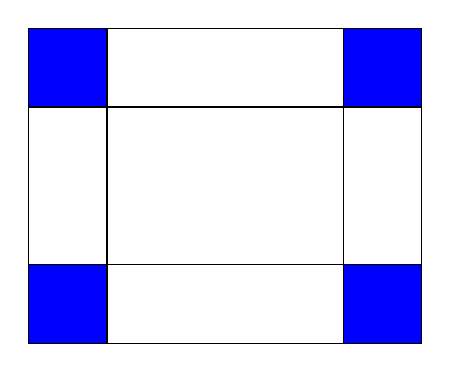
\begin{tikzpicture}[scale=1,font=\footnotesize,line join=round,line cap=round,>=stealth]
				\def  \h{1};
				 \path
					(0,0) coordinate (A)++(0:\h)  coordinate (B)++(0:3*\h) coordinate (C)++(0:\h) coordinate (D)
					(0,\h) coordinate (A')++(0:\h) coordinate (B')++(0:3*\h) coordinate (C')++(0:\h) coordinate (D') 
					(0,3*\h) coordinate (A'')++(0:\h) coordinate  (B'')++(0:3*\h) coordinate (C'')++(0:\h) coordinate (D'')
					(0,4*\h) coordinate (A''')++(0:\h) coordinate (B''')++(0:3*\h) coordinate  (C''')++(0:\h) coordinate (D''');
				\draw  (A) rectangle (D''');
				 \draw (B') rectangle (C'');
				\draw[fill=blue]  (A) rectangle (B');
				\draw[fill=blue] (C) rectangle (D'); 
				\draw[fill=blue] (A'') rectangle  (B''');
				\draw[fill=blue] (C'') rectangle  (D''');
			\end{tikzpicture}
	\end{center}
	Tìm chiều dài của tấm sắt sao cho diện tích  phần còn lại của tấm sắt ít nhất bằng $92$ cm².
	 \loigiai{
		Gọi chiều dài  tấm sắt là $x$ (cm), chiều rộng tấm sắt là $y$ (cm). Điều kiện: $x > 0, y > 0$.\\
		Chu vi hình  chữ nhật $2(x + y) = 48 \Rightarrow y = 24 - x$.\\
		Diện tích tấm  sắt ban đầu \(S_0 = xy = x(24 - x)\).\\
		Diện tích $4$ hình vuông bị cắt đi:  $S_1=4 * 4 = 16$ (cm²).\\
		Diện tích phần còn lại \(S_2 = S_1  - S_2 = x(24 - x) - 16\).\\
		Diện tích phần còn lại ít  nhất 92 cm² nên ta có bất phương trình
		\begin{align*}
			&x(24 - x) - 16 \geq 92\\ \Leftrightarrow &\,  x^2 - 24x + 108 \leq 0\\
			 \Leftrightarrow &\, 6 \le x \le 18.
		\end{align*}
	} 
	Vậy chiều dài của  tấm sắt $x$ với $6 \le x \le 18$.
\end{bt}
